% This is the preamble of a LaTeX source code.
\documentclass[10pt,a4paper]{article}

\setlength{\parskip}{-4pt}%
\setlength{\parindent}{0pt}%

\usepackage{tikz}         % Creating graphics
\usepackage{scrextend}    % KOMA-Script class: labeling
\usepackage{amsfonts}     % Mathematics font: \mathbb

% Needed for busy beaver Turing machine, see
% https://mirror.dogado.de/tex-archive/graphics/pgf/base/doc/pgfmanual.pdß098
% p. 102
\usetikzlibrary {arrows.meta, automata, positioning, shadows}

% Needed for the Turing Machie, see
% https://texample.net//tikz/examples/turing-machine-2/
\usetikzlibrary{chains, fit, shapes}

%...
% \usepackage{multirow} % Required for multirows

% Needed to TM trace, see
% https://stackoverflow.com/questions/1673942/latex-table-positioning
\usepackage{float} % H: Table positioning

% Color list:
\definecolor{amber}{rgb}{1.0, 0.75, 0.0}
\definecolor{amber(sae/ece)}{rgb}{1.0, 0.49, 0.0}
\definecolor{americanrose}{rgb}{1.0, 0.01, 0.24}
\definecolor{amethyst}{rgb}{0.6, 0.4, 0.8}
\definecolor{applegreen}{rgb}{0.55, 0.71, 0.0}
\definecolor{armygreen}{rgb}{0.29, 0.33, 0.13}
\definecolor{coquelicot}{rgb}{1.0, 0.22, 0.0}
\definecolor{english}{rgb}{0.0, 0.5, 0.0}


\begin{document}

\section {Turing machine}

\subsection {Original busy beaver}

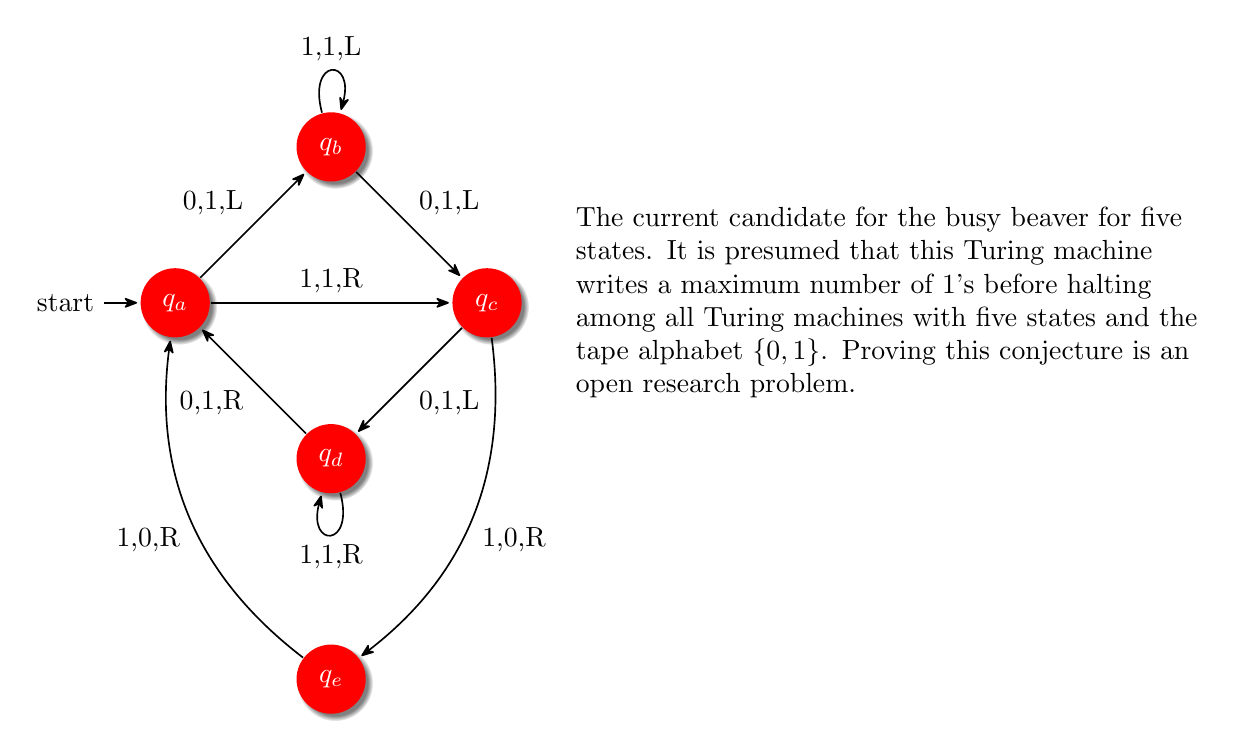
\begin{tikzpicture}[->,>={Stealth[round]},shorten >=1pt,auto,node distance=2.8cm,on grid,semithick,
every state/.style={fill=red,draw=none,circular drop shadow,text=white}]090987
\node[initial,state] (A) {$q_a$};
\node[state] (B) [above right=of A] {$q_b$};
\node[state] (D) [below right=of A] {$q_d$};
\node[state] (C) [below right=of B] {$q_c$};
\node[state] (E) [below=of D] {$q_e$};
\path (A) edge node {0,1,L} (B)
edge node {1,1,R} (C)
(B) edge [loop above] node {1,1,L} (B)
edge node {0,1,L} (C)
(C) edge node {0,1,L} (D)
edge [bend left] node {1,0,R} (E)
(D) edge [loop below] node {1,1,R} (D)
edge node {0,1,R} (A)
(E) edge [bend left] node {1,0,R} (A);
\node [right=1cm,text width=8cm] at (C)
{
The current candidate for the busy beaver for five states. It is
presumed that this Turing machine writes a maximum number of
$1$'s before halting among all Turing machines with five states
and the tape alphabet $\{0, 1\}$. Proving this conjecture is an
open research problem.
};
\end{tikzpicture}


\subsection {Coloured busy beaver}

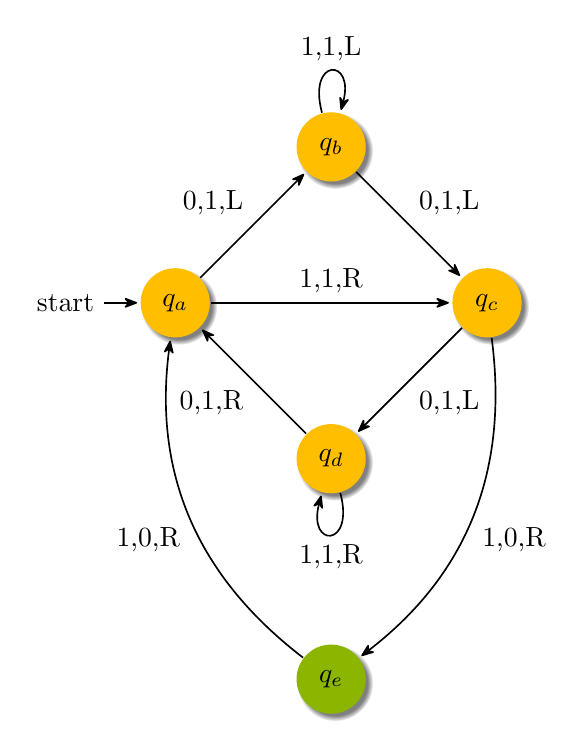
\begin{tikzpicture}[%
    ->,
    >= { Stealth[round] },
    shorten >= 1pt,
    auto,
    node distance = 2.8cm,
    on grid,
    semithick,
    every state/.style = {%
      fill = amber,
      draw = none,
      circular drop shadow,
      text = black }    
  ]
  
\node[initial,state] (A) {$q_a$};
\node[state] (B) [above right=of A] {$q_b$};
\node[state] (D) [below right=of A] {$q_d$};
\node[state] (C) [below right=of B] {$q_c$};
\node[state] (E) [below=of D, fill=applegreen] {$q_e$};

\path
(A) edge node {0,1,L} (B)
edge node {1,1,R} (C)

(B) edge [loop above] node {1,1,L} (B)
edge node {0,1,L} (C)

(C) edge node {0,1,L} (D)
edge [bend left] node {1,0,R} (E)

(D) edge [loop below] node {1,1,R} (D)
edge node {0,1,R} (A)

(E) edge [bend left] node {1,0,R} (A);

\end{tikzpicture}


\section {Preliminary}

\newcommand{\N}{\mathbb{N}} % Set of natural numbers.
\newcommand{\Z}{\mathbb{Z}} % Set of integers.

\subsection {Mathematische Symbole}

\verb+https://oeis.org/wiki/List_of_LaTeX_mathematical_symbols+

\subsection {Menge}

\verb+https://de.wikipedia.org/wiki/Menge_(Mathematik)+
\vskip 8pt

Eine Menge wird über Aufzählung oder Konstuktor - Formel - definiert.

\subsubsection {Aufzählung - Enumeration}

\verb+https://de.wikipedia.org/wiki/Sinn_(Wahrnehmung)+
\vskip 8pt

S oder Sinne: Hören, Riechen, Schmecken, Sehen, Tasten, Temperatur, Schmerz,
Gleichgewicht, Hunger, Durst, Harndrang, $\ldots$ \\
$S = \{ H, R, $\ldots$ \}$
\vskip 8pt
oder
\vskip 8pt
$x$: ist eine Variable von $S$. \\
$|$: ist eine Operation und bedeutet: $x$ kann ein Element oder Wert aus $S$
zugewiesen werden. \\
$S = \{ x\ |\ x = H \lor x = R, \ldots \}$

\subsubsection {Konstruktor - Set builder}

\verb+https://en.wikipedia.org/wiki/Set-builder_notation+
\vskip 8pt

Menge aller natürlichen Zahlen: $\N = \{x \in \N\ |\ x \}$
\vskip 8pt
oder
\vskip 8pt
$\N = \{n\ |\ n \in \N\}$

\vskip 8pt
Menge der ungeraden Integer: $\{n \in \Z\ |\ (\exists k\ [k \in \Z \land n = 2k + 1])\}$
\vskip 8pt
oder
\vskip 8pt
$\{2n + 1\ |\ n \in \Z\}$
\vskip 8pt
und der inverse Konstruktor:
$\{ 2i + 1\ |\ i \in \Z \} = \{ j\ |\ (j - 1) / 2 \in \Z \}$

\subsection {Mengenprodukt}

\verb+https://de.wikipedia.org/wiki/Kartesisches_Produkt+
\vskip 8pt

Das kartesiche Produkt $A \times B$ - ,,A kreuz B'' - zweier Mengen $A$ und $B$
ist die Menge aller geordneten Paare - 2-Tupel oder Liste - $(a, b)$, in denen $a$
ein Element aus $A$ und $b$ ein Element aus $B$ ist:
\vskip 8pt

$A \times B := \{ (a, b)\ |\ a \in A, b \in B \}$


\subsubsection{Beispiel}

$A = \{x, y, z\}$ \\
$B = \{1, 2, 3\}$ \\
$A \times B = \{ (x, 1), (x, 2), (x, 3), (y, 1), (y, 2), (y, 3), (z, 1), (z, 2), (z, 3) \}$


\subsection {Funktion}

\verb+https://en.wikipedia.org/wiki/Function_(mathematics)+ \\
\verb+https://de.wikipedia.org/wiki/Funktion_(Mathematik)+
\vskip 8pt

Eine Funktion oder Abbildung ist eine Beziehung (Relation) zwischen zwei Mengen,
die jedem Element der einen Menge (Funktionsargument: x-Wert) genau ein Element
der anderen Menge (Funktionswert: y-Wert) zuordnet.

\vskip 8pt
Eine Funktion $f$ ordnet jedem Element $x$ einer Definitionsmenge $D$ genau ein
Element $y$ einer Zielmenge $Z$ zu.

\vskip 8pt
\verb+https://mo.mathematik.uni-stuttgart.de/kurse/kurs44/seite25.html+
\vskip 8pt
  \[
  {\bf f: D \rightarrow Z,\ x \mapsto y \hskip 8pt} {\rm oder} \hskip 8pt {\bf f:}
  \left\{%
    \begin{array}{ll}
      {\bf D \rightarrow Z} \\
      {\bf x \mapsto y}
    \end{array}
  \right.
  \]

    
\subsubsection {Notation}

\verb+https://tex.stackexchange.com/questions/87867/do-i-need-a-specific-package-for-n+
\vskip 8pt
\begin{labeling}{Zuordnungsvorschrift mit $D$ und $Z$:} 
  \setlength\itemsep{-3pt}
  \item[Funktionsgleichung:]   $f(x) = x^2,\ x \in \N$
  \item[Zuordnungsvorschrift mit $D$:] $x \rightarrow x^2,\ x \in \N$
    
  \setlength\itemsep{-12pt}
  \item[Zuordnungsvorschrift mit $D$ und $Z$:]
    $f: \N \rightarrow \N,\ x \mapsto x^2$ oder
    \hskip -16pt
    \begin{minipage}{0.3\textwidth}
    \[ f: \left\{%
    \begin{array}{ll}
      \N \rightarrow \N \\
      x \mapsto x^2 
    \end{array}
    \right.
    \]
    \end{minipage}
    
\end{labeling}
\vskip 8pt

\begin{verbatim}
Wertetabelle:
x|1|2|3|...
-----------
y|1|4|9|...
Relation oder Aufzählung: f = {(1,1), (2,4), (3,9), ...}
\end{verbatim}
\vskip 8pt


\subsubsection {Ausdruck}

\verb+https://de.wikipedia.org/wiki/Funktion_(Mathematik)+
\vskip 15pt
\hskip -15pt
\begin{minipage}{0.9\textwidth}
  \begin{itemize}
    \setlength\itemsep{0em}

    \item $x$ wird abgebildet auf $f$ von $x$
    \item $f$ von $x$ wird $x$ eindeutig zugeordnet
    \item $y$ gleich $f$ von $x$
    \item $y$ ist das Bild von $x$ unter der Abbildung $f$
      
  \end{itemize}
\end{minipage}


\subsubsection {Partielle Funktion}

\verb+https://mirror.dogado.de/tex-archive/graphics/pgf/base/doc/pgfmanual.pdf+ \\
\verb+https://de.wikipedia.org/wiki/Partielle_Funktion+ \\
\verb+https://en.wikipedia.org/wiki/Partial_function+ \\
\verb+https://latexdraw.com/exploring-tikz-arrows/+
\vskip 8pt

Eine partielle Funktion ordnet einem Element aus der Menge $X$ ein
Element aus der Menge $Y$ zu.

\vskip 16pt
{\bf Aufzählung}

\vskip 16pt
\begin{verbatim}
X = {1, 2, 3}
Y = {a, b, c, d}
f: X->Y = { 2->d, 3->c}
\end{verbatim}

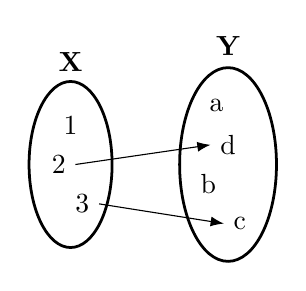
\begin{tikzpicture}

  \node (1) at ( 0.0,   0.5) {1};
  \node (2) at (-0.15,  0.0) {2};
  \node (3) at ( 0.15, -0.5) {3};
  
  \node (a) at (1.85,  0.75) {a};
  \node (d) at (2,     0.25) {d};
  \node (b) at (1.75, -0.25) {b};
  \node (c) at (2.15, -0.75) {c};

  \draw (0, 1.3) node {{\bf X}};
  \draw (2, 1.5)  node {{\bf Y}};
  

  \draw [line width=1pt] (0, 0) ellipse [x radius=15pt, y radius=30pt];
  \draw [line width=1pt] (2, 0) ellipse [x radius=17.5pt, y radius=35pt];

  \draw [-Latex] (2.east) -- (d.west);
  \draw [-Latex] (3.east) -- (c.west);
  
\end{tikzpicture}

\vskip 16pt
{\bf Konstruktion}

\begin{verbatim}
Ungerade natürliche Zahlen.

f: N -> N
f(x) = 2x + 1
\end{verbatim}


\subsection {Algorithmus}

\verb+https://de.wikipedia.org/wiki/Algorithmus+
\vskip 8pt

Ein Algorithmus ist eine Turingmaschine.

\subsubsection {Deterministischer Algorithmus}

\verb+https://de.wikipedia.org/wiki/Determinismus_(Algorithmus)+
\vskip 8pt
Ein Algorithmus ist deterministisch, wenn er für die gleiche Eingabe immer die
gleiche Ausgabe erzeugt und die gleichen Zustände durchlaufen werden.

\subsection {Deterministische Turingmaschine}

\verb+https://de.wikipedia.org/wiki/Turingmaschine+ \\
\verb+https://en.wikipedia.org/wiki/Turing_machine+
\vskip 8pt

Die Zielmenge der partiellen Funktion ersetze ich $\Gamma$ durch $\Sigma$,
um eine Endlosschleife, heutiges Verständnis, zu vermeiden. \\

\noindent
$DTM$ ist eine deterministische Turingmaschine: $<Q, \Gamma, b, \Sigma, \delta, q_0, F >$:
%M=\langle Q,\Gamma ,b,\Sigma ,\delta ,q_{0},F\rangle }M=\langle Q,\Gamma ,b,\Sigma ,\delta ,q_{0},F\rangle

\vskip 15pt
\hskip -15pt
\begin{minipage}{0.9\textwidth}
  \begin{itemize}
    \setlength\itemsep{0em}
    
  \item $\bf Q$ ist eine Zustandsmenge definiert über Aufzählung oder Generator,
    wie z.B. $2k + 1$, weil es sonst zu lange dauert, bis man alle aufgesagt hat,
    wie Zählen.
    
  \item $\bf \Gamma$ ist eine Menge von Speichersymbolen definiert über den
    I/O-Test.
  \item $\bf b \in \Gamma$ ist ein Blank- oder Format-Symbol, das beim Parsen
    ignoriert wird.
  \item $\bf \Sigma \subseteq \Gamma \setminus \{b \}$ ist die Menge der Ausgabesymbole.

    % https://tex.stackexchange.com/questions/47063/rightarrow-vs-implies-and-does-not-imply-symbol:
    % \not \rightarrow
  \item $\bf \delta: (Q \setminus F) \times \Gamma \not \rightarrow Q \times \Sigma \times \{L, R\}$
    ist eine partielle Funktion oder Übergangsfunktion: \\
    $L := Linksbewegung$ (left shift) \\
    $R := Rechtsbewegung$ (right shift) \\
    if $\delta \notin Q$ then $stuck(DTM)$ \\
    Die Übergangsfunktion definiert den Folgezustand, der vom aktuellen Zustand
    abgeleitet wird. Man übersetzt das Eingabesymbol und sucht über eine Tabelle, ob
    der aktuelle Zustand die Eingabe erlaubt. Wenn das nicht zutrifft, stoppt die
    DTM und erzeugt eine Kopie von sich selbst - Core-Dump. \\

    Oder. \\

    Die Übergangsfunktion sagt mir, welchen Nachfolgezustand ich über den
    aktuellen Zustand erreichen kann.

  \item $\bf q_0 \in Q$ ist der Anfangszustand.

  \item $\bf F \subseteq Q$ ist die Menge der Endzustände.
    
  \end{itemize}
\end{minipage}


\subsubsection {Architecture}

\bf {Draft}

\vskip 16pt
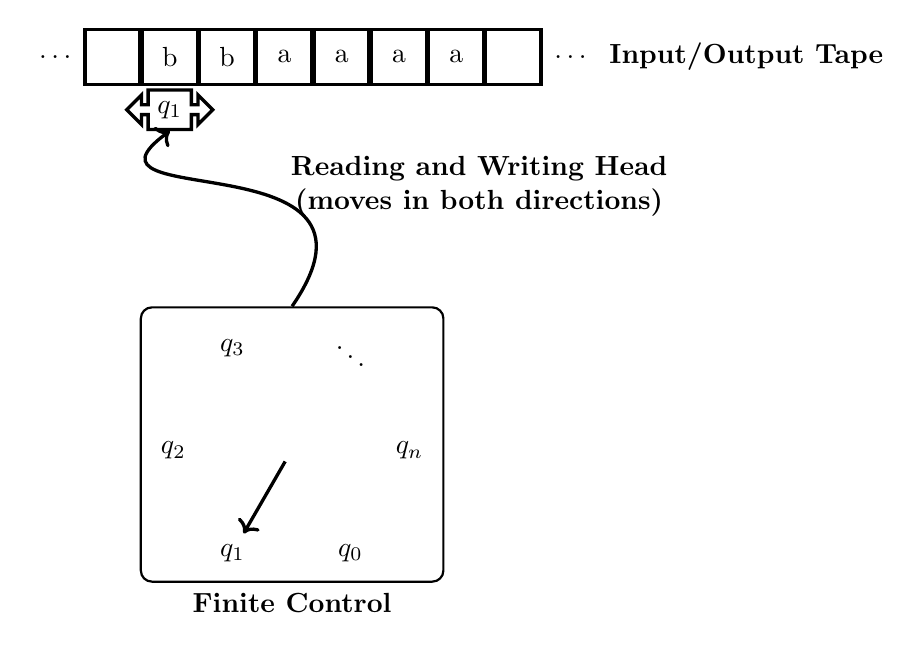
\begin{tikzpicture}
\tikzstyle{every path}=[very thick]

\edef\sizetape{0.7cm}
\tikzstyle{tmtape}=[draw,minimum size=\sizetape]
\tikzstyle{tmhead}=[arrow box,draw,minimum size=.5cm,arrow box
  arrows={east:.25cm, west:0.25cm}]

%% Draw TM tape
\begin{scope}[start chain=1 going right,node distance=-0.15mm]
    \node [on chain=1,tmtape,draw=none] {$\ldots$};
    \node [on chain=1,tmtape] {};
    \node [on chain=1,tmtape] (input) {b};
    \node [on chain=1,tmtape] {b};
    \node [on chain=1,tmtape] {a};
    \node [on chain=1,tmtape] {a};
    \node [on chain=1,tmtape] {a};
    \node [on chain=1,tmtape] {a};
    \node [on chain=1,tmtape] {};
    \node [on chain=1,tmtape,draw=none] {$\ldots$};
    \node [on chain=1] {\textbf{Input/Output Tape}};
\end{scope}

%% Draw TM Finite Control
\begin{scope}
[shift={(3cm,-5cm)},start chain=circle placed {at=(-\tikzchaincount*60:1.5)}]
\foreach \i in {q_0,q_1,q_2,q_3,\ddots,q_n}
	\node [on chain] {$\i$};

% Arrow to current state
\node (center) {};
\draw[->] (center) -- (circle-2);

\node[rounded corners,draw=black,thick,fit=(circle-1) (circle-2) (circle-3) 
      (circle-4) (circle-5) (circle-6),
			label=below:\textbf{Finite Control}] (fsbox)
		{};
\end{scope}

%% Draw TM head below (input) tape cell
\node [tmhead,yshift=-.3cm] at (input.south) (head) {$q_1$};

%% Link Finite Control with Head
\path[->,draw] (fsbox.north) .. controls (4.5,-1) and (0,-2) .. node[right] 
			(headlinetext)
 			{} 
			(head.south);
\node[xshift=3cm] at (headlinetext)  
			{\begin{tabular}{c} 
				\textbf{Reading and Writing Head} \\  
				\textbf{(moves in both directions)} 
			 \end{tabular}};
\end{tikzpicture}


\vskip 16pt
\bf {CPU}
\vskip 16pt


\subsection{Busy beaver}

\verb+https://en.wikipedia.org/wiki/Turing_machine+

\vskip 8pt
{\bf Legend}
  
\vskip 4pt
\begin{labeling}{\rm P $:=$ } 
  \setlength\itemsep{-3pt}
  \item[\rm P $:=$] \rm Program counter
  \item[S $:=$] Start or initial state
  \item[C $:=$] Current state
  \item[I $:=$] Input
  \item[O $:=$] Output
  \item[A $:=$] ALU
  \item[N $:=$] Next state
  \item[M $:=$] Memory state
\end{labeling}

\vskip 8pt
{\bf DTM}
  
\vskip 15pt
\hskip -15pt
\begin{minipage}{0.9\textwidth}
  \begin{itemize}
    \setlength\itemsep{0em}
    
  \item $Q = \{ A, B, C, H \}$
  \item $\Gamma = \{ 0, 1 \}$
  \item $b = 0$
  \item $\Sigma = \{ 1 \}$
  \item $q_0 = S = A$
  \item $F = \{ H \}$ 
    
  \end{itemize}
\end{minipage}

\subsubsection{States}
\verb+http://www.cs.uni.edu/~barr/CS1000/ppt/Chapter09-ComputerOperation.pdf+
\verb+https://en.wikipedia.org/wiki/Address_generation_unit+

\vskip 8pt
{\bf A} $:=$ \rm Arithmetical logical unit including AGU
- address generation unit - with the micro operations:
$read, \ calculate,\ write,\ address$ \\
{\bf R} $:=$ Right address \\
{\bf L} $:=$ Left address \\
{\bf S} $:=$ Stop or stay on the same address

\newcommand\tb[1] {\textbf{#1}}
\newcommand\e[1] {\colorbox{amber}{\bf #1}}

\vskip 4pt
% https://latex-tutorial.com/tutorials/tables/
%
\begin{table}[H]
  \begin{center}
    \begin{tabular}{|c|c|c|c|c|}
      \hline
      % <-- added & and content for each colum
      \tb{C} & \tb{I} & \tb{O} & \tb{A} & \tb{N}\\ % <--
      S & 0 & 0 & S & A \\ % <--      
      \hline
      A & 0 & 1 & R & B \\ % <--      
      A & 1 & 1 & L & C \\ % <--      
      \hline
      B & 0 & 1 & L & A \\ % <--      
      B & 1 & 1 & R & B \\ % <--      
      \hline
      C & 0 & 1 & L & B \\ % <--      
      C & 1 & 1 & R & H \\ % <--      
      \hline
      H & 1 & 1 & S & H \\ % <--      
      \hline
    \end{tabular}
  \end{center}
\end{table}


\subsubsection{Trace}

\vskip 16pt
{\bf Log}
       
\vskip 4pt
% https://latex-tutorial.com/tutorials/tables/
%
\begin{table}[H]
  \begin{center}
    \begin{tabular}{|c|c|c|c|c|c|c|}
      \hline
      % <-- added & and content for each colum
      \tb{P} & \tb{C} & \tb{I} & \tb{O} & \tb{A} & \tb{N} & \tb{M}\\ % <--
      \hline
      0  & S & 0 & 0 & S & A & $\{0, \ldots$, 0,    0,    0,    0, \e 0,    0,    0,    0, $\ldots, 0\}$\\ % <--      
      1  & A & 0 & 1 & R & B & $\{0, \ldots$, 0,    0,    0,    0,    1, \e 0,    0,    0, $\ldots, 0\}$\\ % <--      
      2  & B & 0 & 1 & L & A & $\{0, \ldots$, 0,    0,    0,    0, \e 1,    1,    0,    0, $\ldots, 0\}$\\ % <--
      3  & A & 1 & 1 & L & C & $\{0, \ldots$, 0,    0,    0, \e 0,    1,    1,    0,    0, $\ldots, 0\}$\\ % <--      
      4  & C & 0 & 1 & L & B & $\{0, \ldots$, 0,    0, \e 0,    1,    1,    1,    0,    0, $\ldots, 0\}$\\ % <--      
      5  & B & 0 & 1 & L & A & $\{0, \ldots$, 0, \e 0,    1,    1,    1,    1,    0,    0, $\ldots, 0\}$\\ % <--      
      6  & A & 0 & 1 & R & B & $\{0, \ldots$, 0,    1, \e 1,    1,    1,    1,    0,    0, $\ldots, 0\}$\\ % <--      
      7  & B & 1 & 1 & R & B & $\{0, \ldots$, 0,    1,    1, \e 1,    1,    1,    0,    0, $\ldots, 0\}$\\ % <--      
      8  & B & 1 & 1 & R & B & $\{0, \ldots$, 0,    1,    1,    1, \e 1,    1,    0,    0, $\ldots, 0\}$\\ % <--      
      9  & B & 1 & 1 & R & B & $\{0, \ldots$, 0,    1,    1,    1,    1, \e 1,    0,    0, $\ldots, 0\}$\\ % <--      
      10 & B & 1 & 1 & R & B & $\{0, \ldots$, 0,    1,    1,    1,    1,    1, \e 0,    0, $\ldots, 0\}$\\ % <--      
      11 & B & 0 & 1 & L & A & $\{0, \ldots$, 0,    1,    1,    1,    1, \e 1,    0,    0, $\ldots, 0\}$\\ % <--      
      12 & A & 1 & 1 & L & C & $\{0, \ldots$, 0,    1,    1,    1, \e 1,    1,    0,    0, $\ldots, 0\}$\\ % <--      
      13 & C & 1 & 1 & R & H & $\{0, \ldots$, 0,    1,    1, \e 1,    1,    1,    0,    0, $\ldots, 0\}$\\ % <--
      14 & H & 1 & 1 & S & H & $\{0, \ldots$, 0,    1,    1, \e 1,    1,    1,    0,    0, $\ldots, 0\}$\\ % <--
      \hline
    \end{tabular}
  \end{center}
\end{table}


\vskip 16pt
\begin{description}
  
\item[Beobachtung:]
In der Berufsschule verwendet man bunte Begriffe, die man
2-dimensionalen mit z.T. bidrektionen Pfeilen verbindet und
zwar unspezifiert.

\item[Idee:]
Das ist ein Algorithmus und ein Automat.
Als Modell verwende ich deterministische Turing Maschine,
damit es nicht zu kompliziert wird.

\item[Spiel:]
Jeder Mensch, Mathematiker oder Philosoph spielt dauernd mit irgendwelchen Zeichen:

\item[xxx: ]
Um alles zu vereinfachen, beschränke ich mich auf eine
deterministische Turing Maschine - DTM - oder einen Computer, der das macht,
was - tbd. - er laut Beschreibung kann und zwar sofort - tbd. - ein Ergebnis
sofort liefert, das mit der Erwartiung übereinstimmt.

\item[xxx: ]
Ziemlich frei habe ich alles umdefininiert:

DTM = (C, I, R, B, F, T, S)
\end{description}
  
\begin{description}
\item[C := ] States of the computer
\item[I := ] I/O characters (abstract)
\item[M := ] Memory
\item[B := ] Power on or boot phase
\item[F := ] Functions
\item[T := ] Timeout actions like powersaveing
\item[S := ] Power off or shutdown
\end{description}



\vskip 20pt
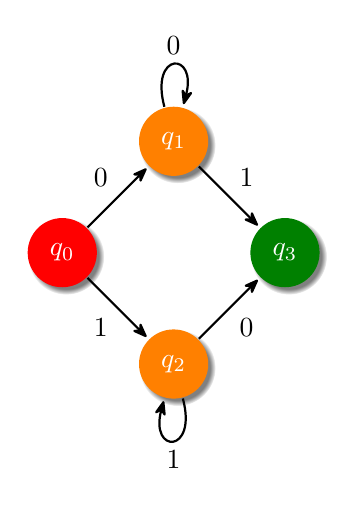
\begin{tikzpicture} [%
    shorten >= 1pt,
    node distance = 2cm,
    on grid,
    >= {Stealth[round]},
    thick,    
    every state/.style = {%
      fill,draw = none,orange,
      text = white,
      circular drop shadow },    
    accepting/.style ={%
      green!50!black,
      text = white },    
    initial/.style ={%
      red, text = white}
  ]
  
\node[state,initial]    (q_0) {$q_0$};
\node[state]            (q_1) [above right=of q_0] {$q_1$};
\node[state]            (q_2) [below right=of q_0] {$q_2$};
\node[state,accepting]  (q_3) [below right=of q_1] {$q_3$};

\path[->]
(q_0) edge node [above left] {0} (q_1)
edge node [below left] {1} (q_2)

(q_1) edge node [above right] {1} (q_3)
edge [loop above] node {0} ()

(q_2) edge node [below right] {0} (q_3)
edge [loop below] node {1} ();

\end{tikzpicture}

\section {Derivation}

\subsection{Legend}

\begin{labeling}{\color{applegreen}{\bf Applegreen:}}
  \setlength\itemsep{-3pt}
\item[\color{applegreen}{\bf Applegreen:}] initial state
\item[\color{amber}{\bf Amber:}]           any state
\item[\color{coquelicot}{\bf Coquelicot:}] final state
\end{labeling}


\subsection{Subject - Deadline}

\begin{labeling}{\bf 2. Deadline - p:} 
  \setlength\itemsep{-3pt}
\item[\bf 1. Subject - s:]  Die Tractatus Dimensionen oder wie alle in jedem Kosmos denken
\item[\bf 2. Deadline - d:] 23.12.2022
\end{labeling}

\begin{verbatim}
Draft:
s <-> d
\end{verbatim}

\vskip 8pt
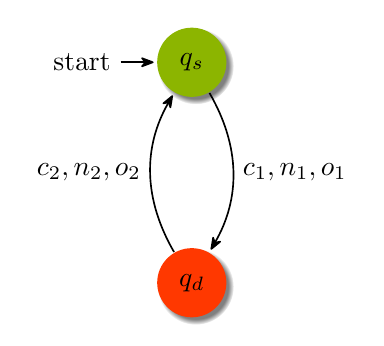
\begin{tikzpicture} [%
    ->,
    >= { Stealth[round] },
    shorten >= 1pt,
    auto,
    node distance = 2.8cm,
    on grid,
    semithick,
    every state/.style = {%
      fill = amber,
      draw = none,
      circular drop shadow,
      text = black }    
  ]

  \node[initial, state, fill=applegreen] (S) {$q_s$};
  \node[state] (D) [below=of S, fill=coquelicot] {$q_d$};

  \path
  (S) edge [bend left] node {$c_1,n_1,o_1$} (D)
  (D) edge [bend left] node {$c_2,n_2,o_2$} (S);
  
\end{tikzpicture}

\subsection{Proposition}

\begin{labeling}{\bf 2. Proposition - p:} 
  \setlength\itemsep{-3pt}
\item[\bf 1. Subject - s:]     Die Tractatus Dimensionen oder wie alle in jedem
  Kosmos denken
\item[\bf 2. Proposition - p:] Literate Programming / LuaTeX
\item[\bf 3. Deadline - p:]    23.12.2022
\end{labeling}

\begin{verbatim}
Draft:
s -> l(p) -> d
\end{verbatim}

\vskip 16pt
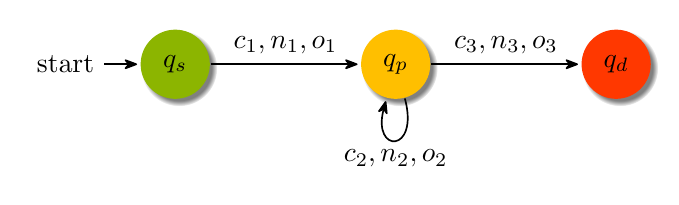
\begin{tikzpicture} [%
    ->,
    >= { Stealth[round] },
    shorten >= 1pt,
    auto,
    node distance = 2.8cm,
    on grid,
    semithick,
    every state/.style = {%
      fill = amber,
      draw = none,
      circular drop shadow,
      text = black }    
  ]

  \node[initial, state, fill=applegreen] (S) {$q_s$};
  \node[state] (P) [right=of S] {$q_p$};
  \node[state] (D) [right=of P, fill=coquelicot] {$q_d$};

  \path
  (S) edge node {$c_1,n_1,o_1$} (P)
  (P) edge [loop below] node {$c_2,n_2,o_2$} (P)
  (P) edge node {$c_3,n_3,o_3$} (D);
  
\end{tikzpicture}


\subsection{Knowledge}

\begin{labeling}{\bf 2. Proposition - p:} 
  \setlength\itemsep{-3pt}
\item[\bf 1. Subject - s:]     Die Tractatus Dimensionen oder wie alle in jedem
  Kosmos denken
\item[\bf 2. Knowledge - k:]   Rezitation des Tractatus

\item[\bf 3. Proposition - p:] Literate Programming / LuaTeX
\item[\bf 4. Deadline - p:]    23.12.2022
\end{labeling}

\begin{verbatim}
Draft:
     -> l(k) <-
    |          |
    s          v
              l(p)
               |
           d <-
\end{verbatim}

\vskip 16pt
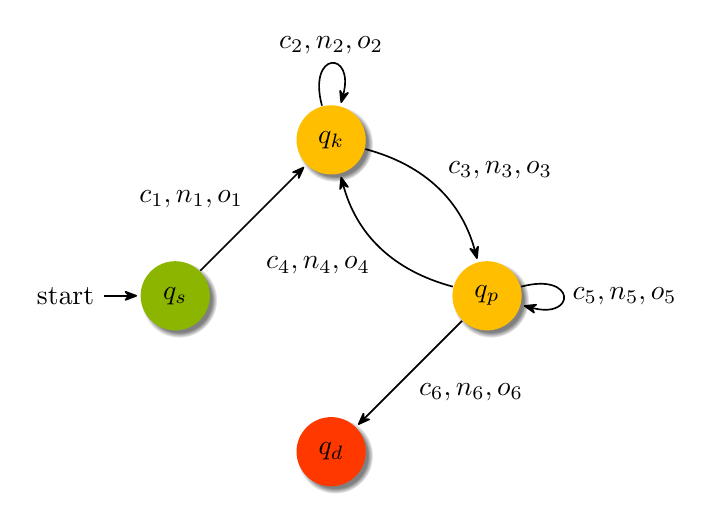
\begin{tikzpicture} [%
    ->,
    >= { Stealth[round] },
    shorten >= 1pt,
    auto,
    node distance = 2.8cm,
    on grid,
    semithick,
    every state/.style = {%
      fill = amber,
      draw = none,
      circular drop shadow,
      text = black }    
  ]

  \node[initial, state, fill=applegreen] (S) {$q_s$};
  \node[state] (K) [above right=of S] {$q_k$};
  \node[state] (P) [below right=of K] {$q_p$};
  \node[state] (D) [below right=of S, fill=coquelicot] {$q_d$};
  
  \path
  (S) edge node {$c_1,n_1,o_1$} (K)
  
  (K) edge [loop above] node {$c_2,n_2,o_2$} (K)
  edge [bend left] node {$c_3,n_3,o_3$} (P)

  (P) edge [bend left] node {$c_4,n_4,o_4$} (K)
  edge [loop right] node {$c_5,n_5,o_5$} (P)

  (P) edge node {$c_6,n_6,o_6$} (D);
  ;
  
\end{tikzpicture}


\begin{verbatim}

Contents

1. Subject - s:     Die Tractatus Dimensionen
                    oder wie alle im Weltall denken
2. Knowledge - k:   Rezitation des Tractatus
3. Proposition - p: Literate Programming / LuaTeX
4. Deadline - d:    23.12.2022
5. Hypothesis - h:  i. Begriffe sind Koordinatenachsen

Legend:
Eine Landkarte versteht man über eine
Übersetzung.
https://de.wikipedia.org/wiki/Legende_(Karte)

Colors:
Wenn man die Ampelfarben nicht versteht,
kann man ganz schnell sterben.

htps://de.wikipedia.org/wiki/Ampel

1. s <-> d

2. s -> l(p) -> d

3.   -> l(k) <-
    |          |
    s          v
              l(p)
               |
           d <-

4.   -> l(k) <-
    |          |
    s          v
              l(p)
               |
           d <-

\end{verbatim}

\end{document}
